\documentclass[aspectratio=169]{beamer}
\usepackage[utf8]{inputenc}
\usepackage{amsmath, amssymb, amsthm}
\usepackage{graphicx}

\title{Trace and Spectral Norms of Tensor Powers \\ using Krylov Subspace Methods}
\author{Martin Juhász}
\date{}

\begin{document}

\begin{frame}
  \titlepage
\end{frame}

\begin{frame}{Introduction \& Motivation}
  \begin{itemize}
    \item The \textbf{Schatten $p$-norm} of $A \in \mathbb{C}^{N \times N}$ is the $\ell_p$-norm of its singular values:
      \begin{equation*}
        \|A\|_p = \left( \sum_{i=1}^N \sigma_i^p \right)^{1/p}
      \end{equation*}
    \item $p=1 \implies$ Trace Norm
    \item $p \to \infty \implies$ Spectral Norm (largest singular value)
    \item \textbf{The Challenge:} Computing exact norms requires Singular Value Decomposition (SVD), which costs $\mathcal{O}(N^3)$ time and $\mathcal{O}(N^2)$ memory.
  \end{itemize}
\end{frame}

\begin{frame}{Target Operator \& The Tensor Wall}
  \begin{itemize}
    \item Our focus is on evaluating linear combinations of Kronecker powers:
      \begin{equation*}
        M = c_1 A^{\otimes n} + c_2 B^{\otimes n}
      \end{equation*}
    \item For $3 \times 3$ building blocks, the dimension grows exponentially: \textbf{$N = 3^n$}.
    \item The spectrum of such tensor networks is highly structured but rugged/clustered, causing standard decomposition solvers to stagnate or fail.
    \item Exact dense SVD becomes utterly uncomputable past $n=9$ due to memory constraints.
  \end{itemize}
\end{frame}

\begin{frame}{Generalized Matrix Functions}
  \begin{itemize}
    \item Instead of full SVD, we treat the norm estimation via \textit{generalized matrix functions} ($f^\diamond(M) = U f(\Sigma) V^\dagger$).
    \item The trace norm ($p=1$) is equivalent to evaluating the trace of $\sqrt{M^\dagger M}$:
      \begin{equation*}
        \|M\|_1 = \mathrm{tr}\left( \sqrt{M^\dagger M} \right)
      \end{equation*}
    \item \textbf{Hutchinson's trace estimator} approximates this trace using $s$ random vectors $v_i$:
      \begin{equation*}
        \mathrm{tr}\left( \sqrt{M^\dagger M} \right) \approx \frac{1}{s} \sum_{i=1}^s v_i^\dagger \sqrt{M^\dagger M} v_i
      \end{equation*}
  \end{itemize}
\end{frame}

\begin{frame}{Matrix-Free Krylov Projection \& Quadrature}
  \begin{itemize}
    \item Applying the Lanczos algorithm to an operator generates orthogonal polynomials with respect to its spectral measure.
    \item By projecting onto a low-dimensional Krylov subspace, we obtain a tridiagonal matrix $T_\ell$.
    \item Evaluating the matrix function on $T_\ell$ is mathematically equivalent to an $\ell$-point \textbf{Gaussian quadrature rule} over the spectral distribution.
    \item \textbf{Matrix-Free Advantage:} We only need an abstract subroutine for matrix-vector products $y \leftarrow M x$. The massive $N \times N$ matrix is never explicitly stored!
  \end{itemize}
\end{frame}

\begin{frame}{Golub-Kahan Bidiagonalization (GKB)}
  \begin{itemize}
    \item \textbf{Numerical Stability Issue:} Applying Lanczos directly to $M^\dagger M$ squares the condition number, leading to rapid loss of orthogonality.
    \item \textbf{Solution:} Project $M$ directly using GKB, building bases $U_\ell$ and $V_\ell$:
      \begin{equation*}
        M V_\ell = U_\ell B_\ell, \quad M^\dagger U_\ell = V_\ell B_\ell^\dagger + \gamma_\ell u_{\ell+1} e_\ell^T
      \end{equation*}
    \item The singular values of the small bidiagonal matrix $B_\ell$ serve exactly as the Gaussian quadrature nodes.
    \item \textbf{3-Term Recurrence:} GKB only needs the current, previous, and next vectors. The memory footprint remains strictly bounded at $\mathbf{\mathcal{O}(N)}$.
    \item \begin{equation*}
        v^\dagger \sqrt{M^\dagger M} v \approx \|v\|_2^2 \left[ \sqrt{B_\ell^\dagger B_\ell} \right]_{1,1}
      \end{equation*}
  \end{itemize}
\end{frame}

\begin{frame}{Spectral Norm \& IRLM}
  \begin{itemize}
    \item For the spectral norm ($p=\infty$), we strictly seek the maximum singular value.
    \item Hutchinson stochastic averaging is completely unnecessary for this.
    \item We apply \textbf{Implicitly Restarted Lanczos Method (IRLM)} directly.
    \item The algorithm extracts \textbf{Ritz values} that dynamically approximate the extreme eigenvalues.
    \item IRLM converges exceptionally fast and is significantly more computationally efficient than a full GKB projection.
  \end{itemize}
\end{frame}

\begin{frame}{Accuracy Verification: Trace Norm ($n=8$)}
  \begin{itemize}
    \item Exact ground-truths acquired via SU(3) block-diagonal representations (\texttt{tensorpow}).
    \item At $n=8$ ($N=6,561$), convergence is sufficient using chosen $s$ and $m$ bounds.
  \end{itemize}
  \begin{center}
    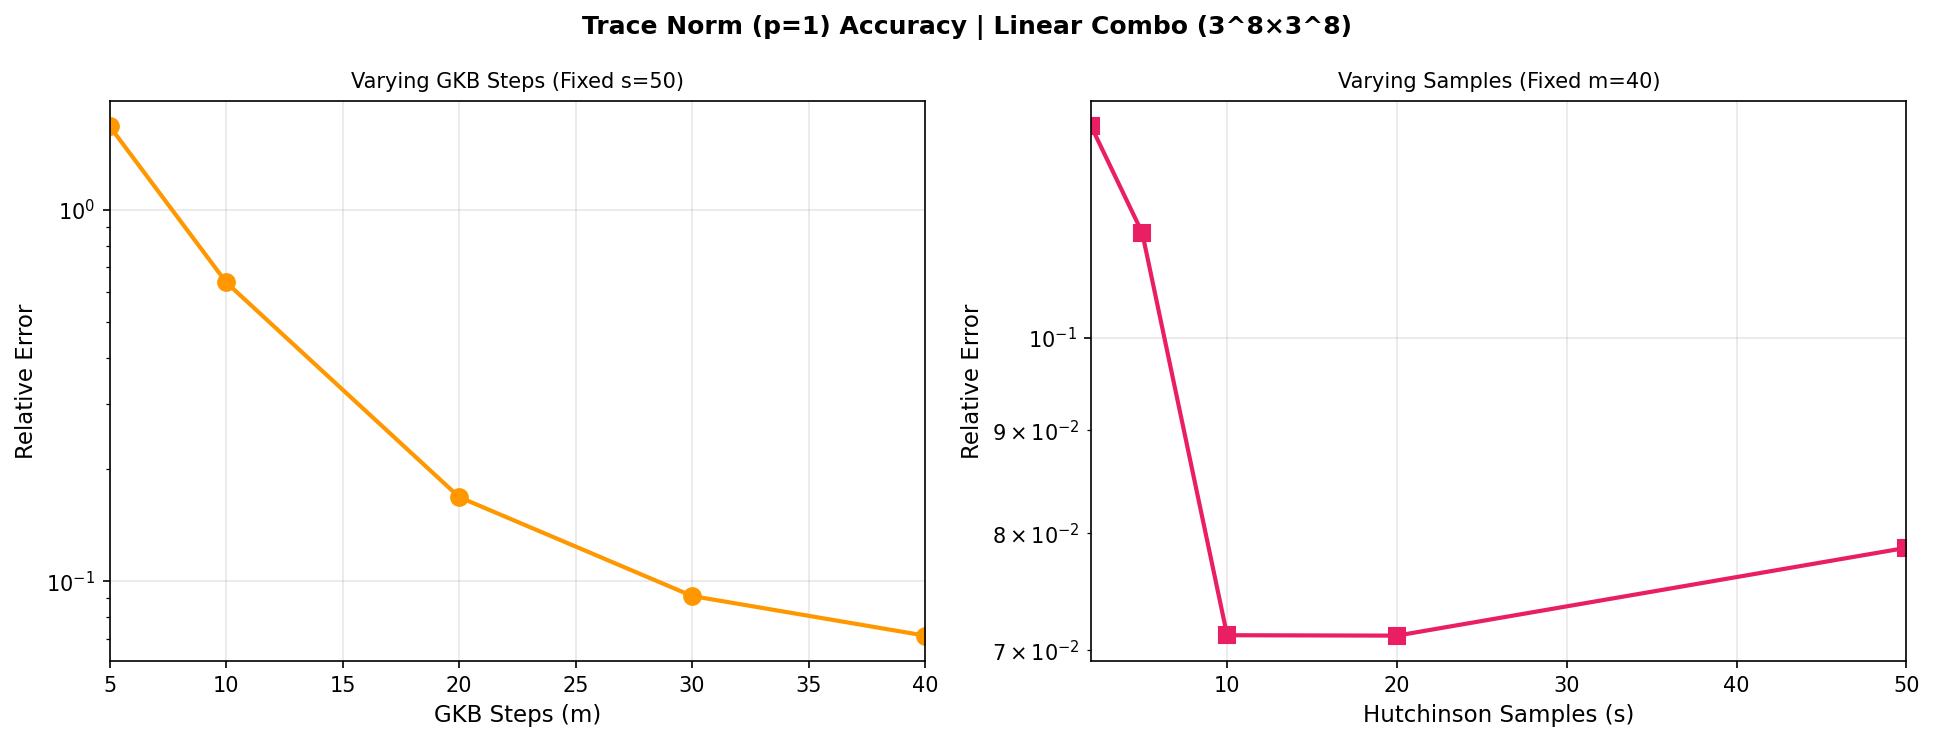
\includegraphics[height=0.65\textheight]{accuracy_n8_p1.png}
  \end{center}
\end{frame}

\begin{frame}{Accuracy Verification: Spectral Norm ($n=8$)}
  \begin{itemize}
    \item The spectral norm converges rapidly using the Implicitly Restarted Lanczos Method.
  \end{itemize}
  \begin{center}
    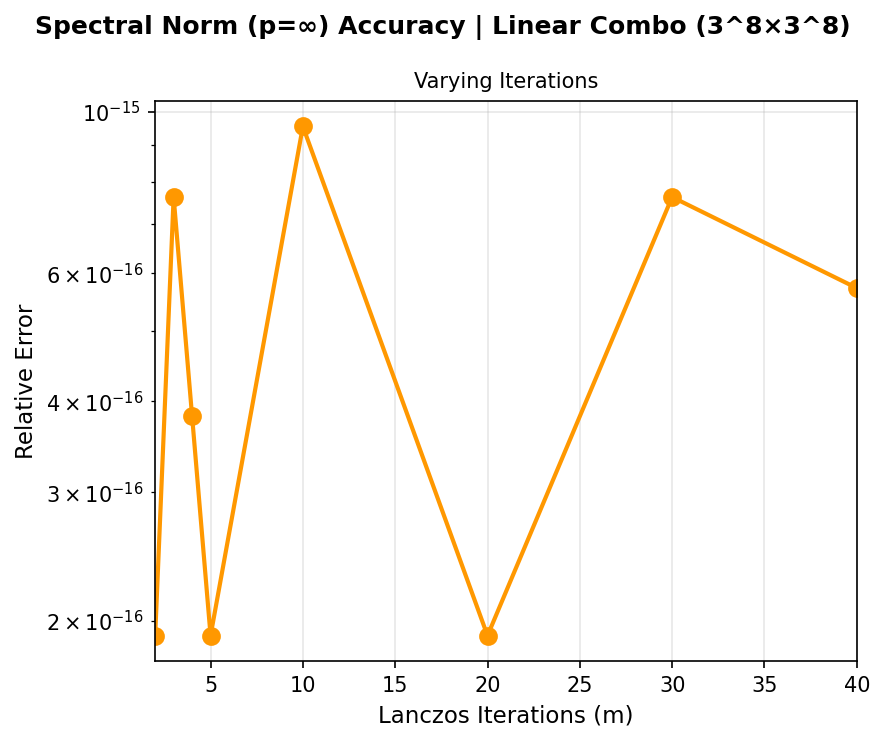
\includegraphics[height=0.65\textheight]{accuracy_n8_pinf.png}
  \end{center}
\end{frame}

\begin{frame}{Accuracy Scaling: Trace Norm ($n=11$)}
  \begin{itemize}
    \item At $n=11$ ($N=177,147$), the error for $p=1$ remains unacceptably high, indicating $s$ and $m$ must be increased.
  \end{itemize}
  \begin{center}
    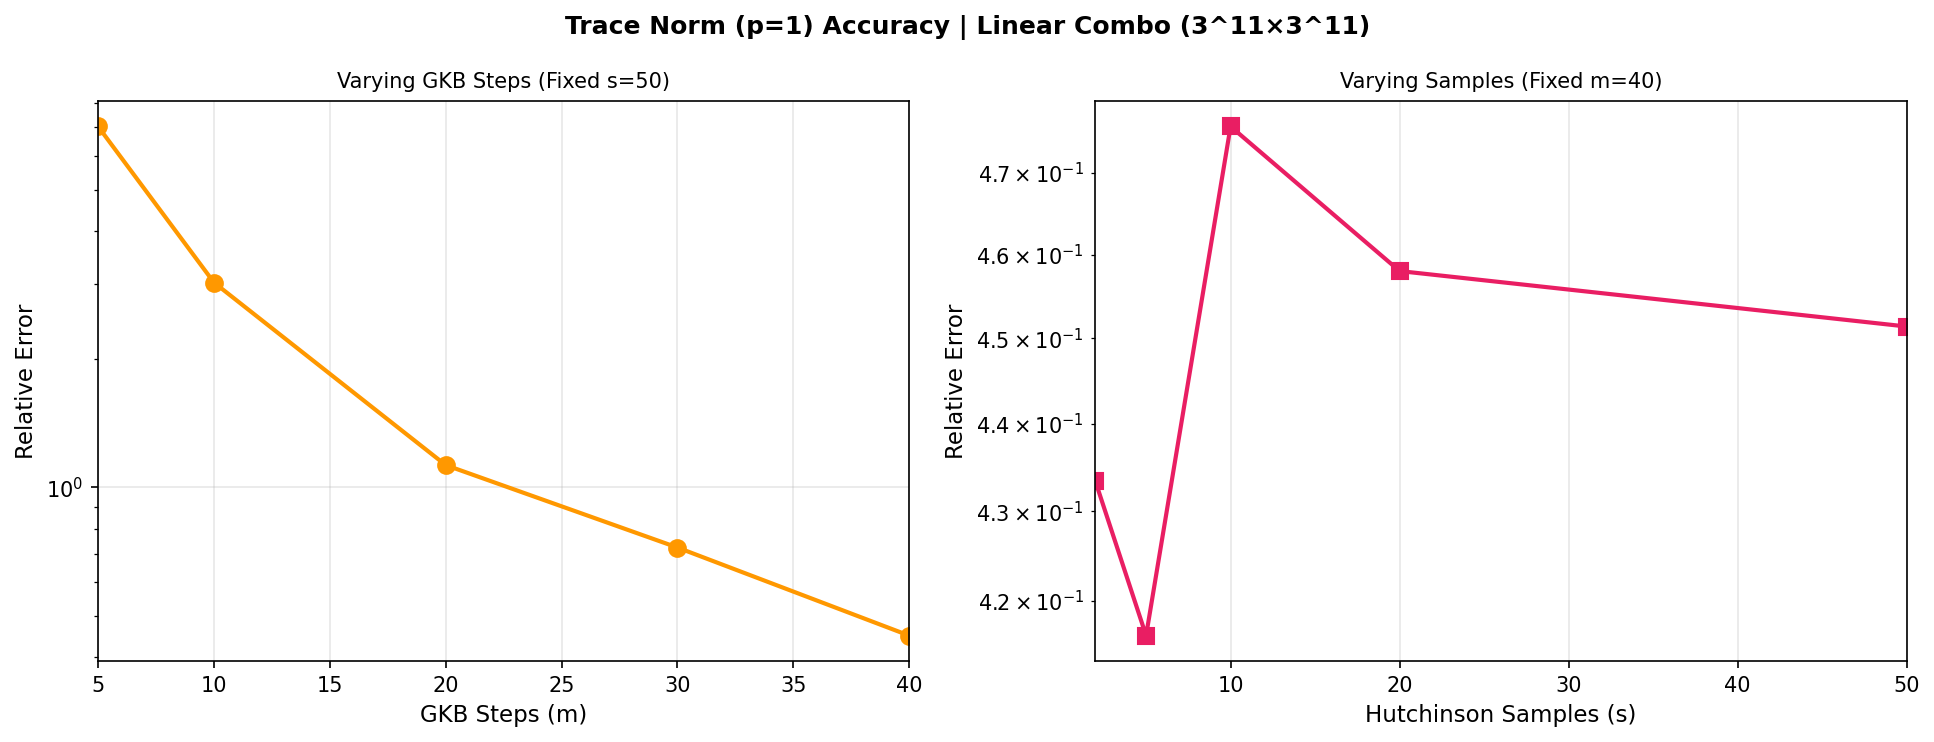
\includegraphics[height=0.65\textheight]{accuracy_n11_p1.png}
  \end{center}
\end{frame}

\begin{frame}{Accuracy Scaling: Spectral Norm ($n=11$)}
  \begin{itemize}
    \item The spectral norm continues to converge efficiently for larger tensor powers.
  \end{itemize}
  \begin{center}
    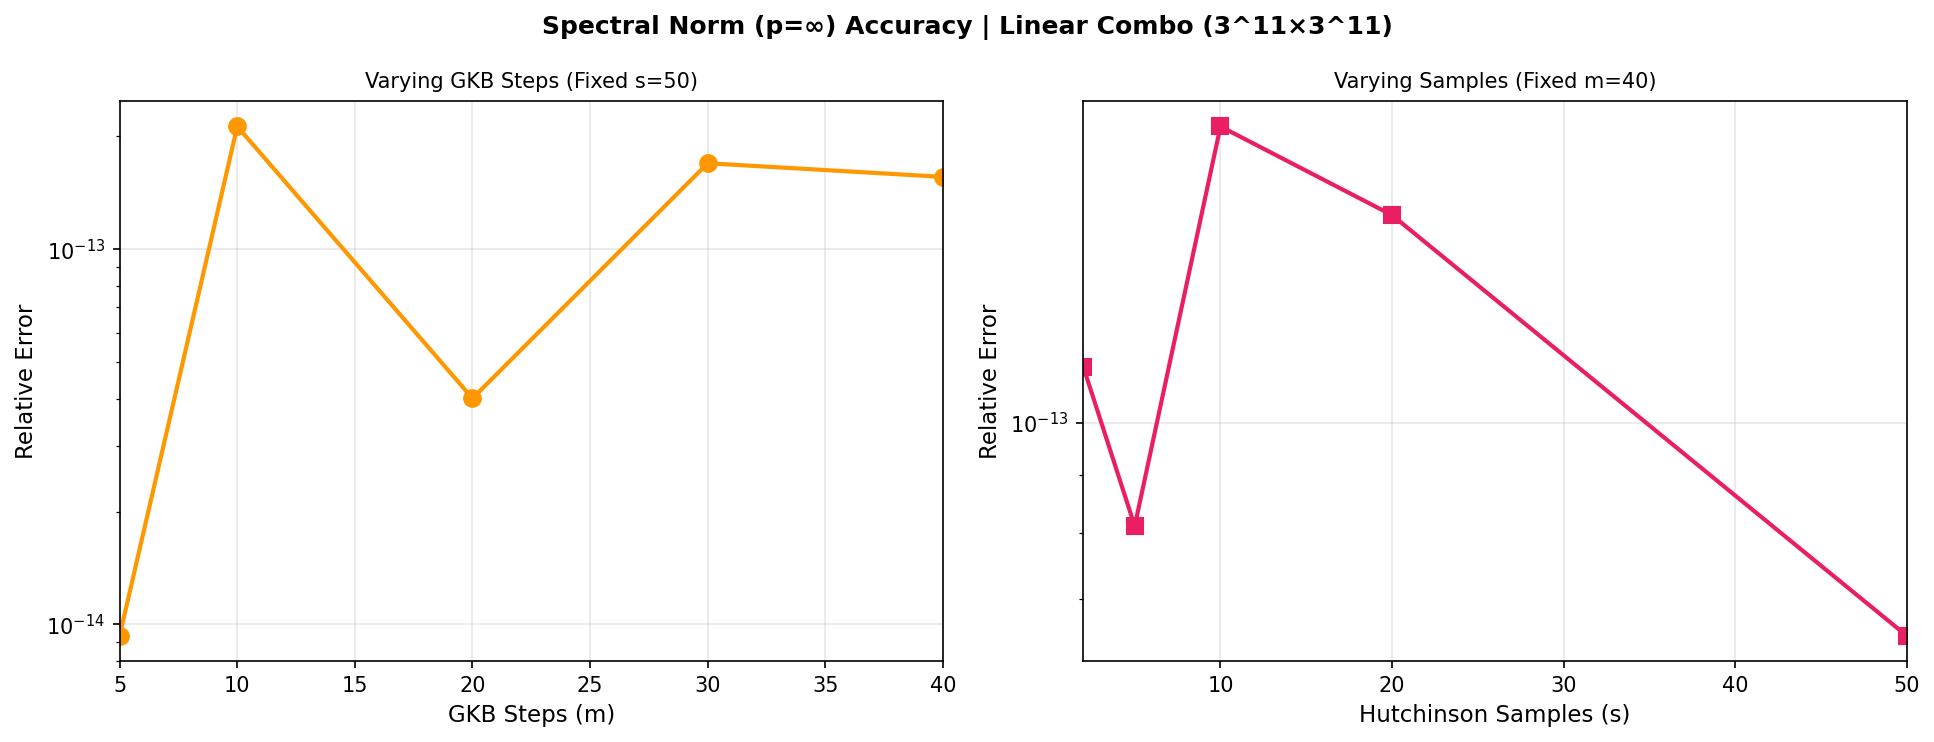
\includegraphics[height=0.65\textheight]{accuracy_n11_pinf.png}
  \end{center}
\end{frame}

\begin{frame}{Performance Scaling Breakthrough: Computation Time}
  \begin{itemize}
    \item Dense SVD takes 40 mins at $n=9$. Krylov methods scale with $\mathcal{O}(N)$ instead of $\mathcal{O}(N^3)$.
  \end{itemize}
  \begin{center}
    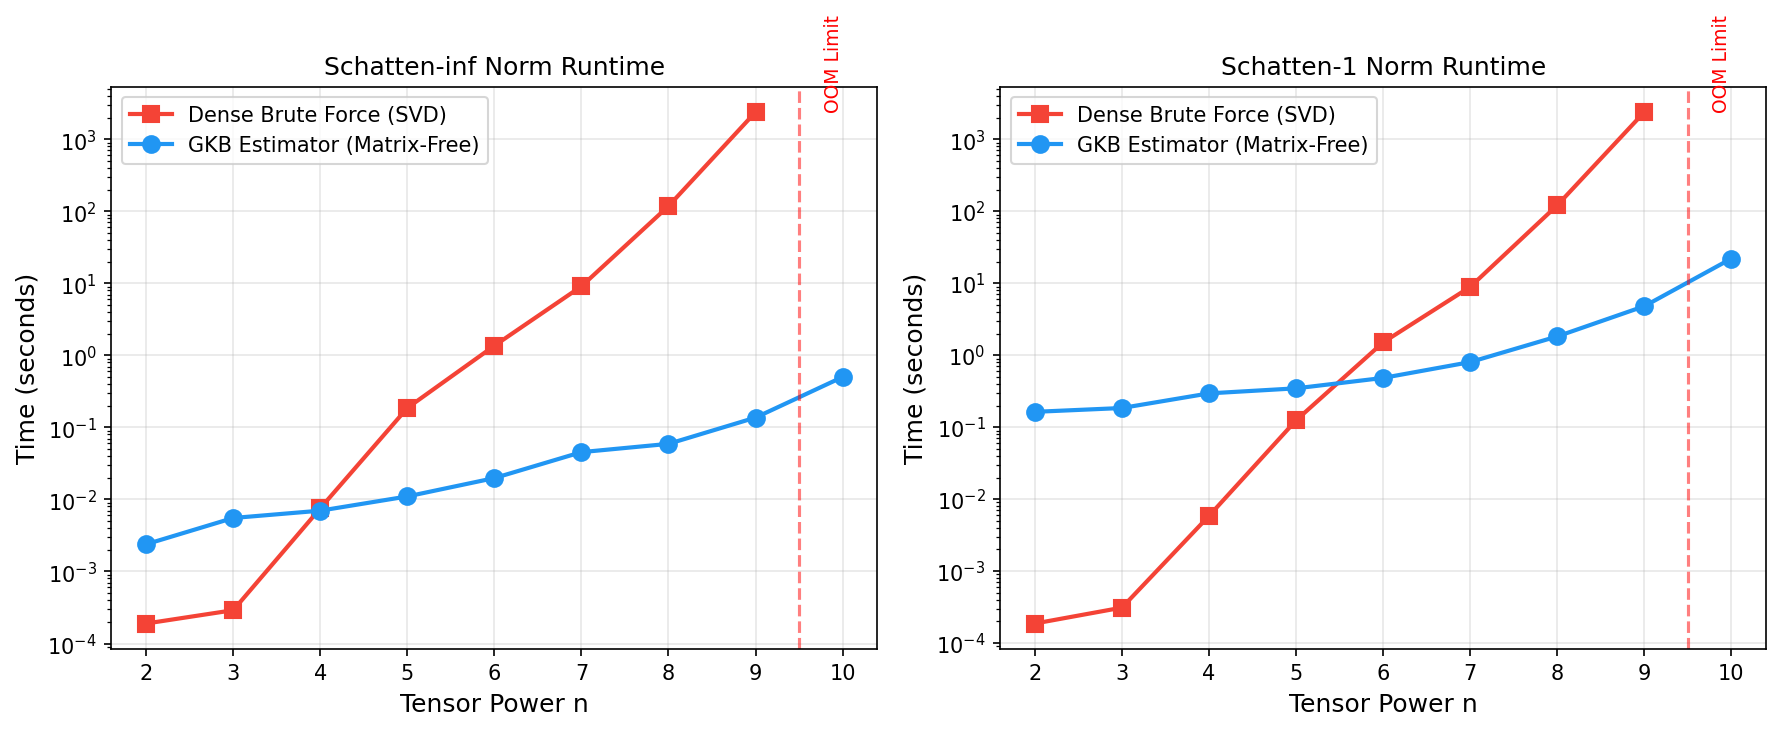
\includegraphics[height=0.65\textheight]{speed_comparison.png}
  \end{center}
\end{frame}

\begin{frame}{Performance Scaling Breakthrough: Peak Memory}
  \begin{itemize}
    \item Dense SVD triggers OOM at $n=10$. The GKB matrix-free memory footprint remains bounded at $\mathcal{O}(N)$.
  \end{itemize}
  \begin{center}
    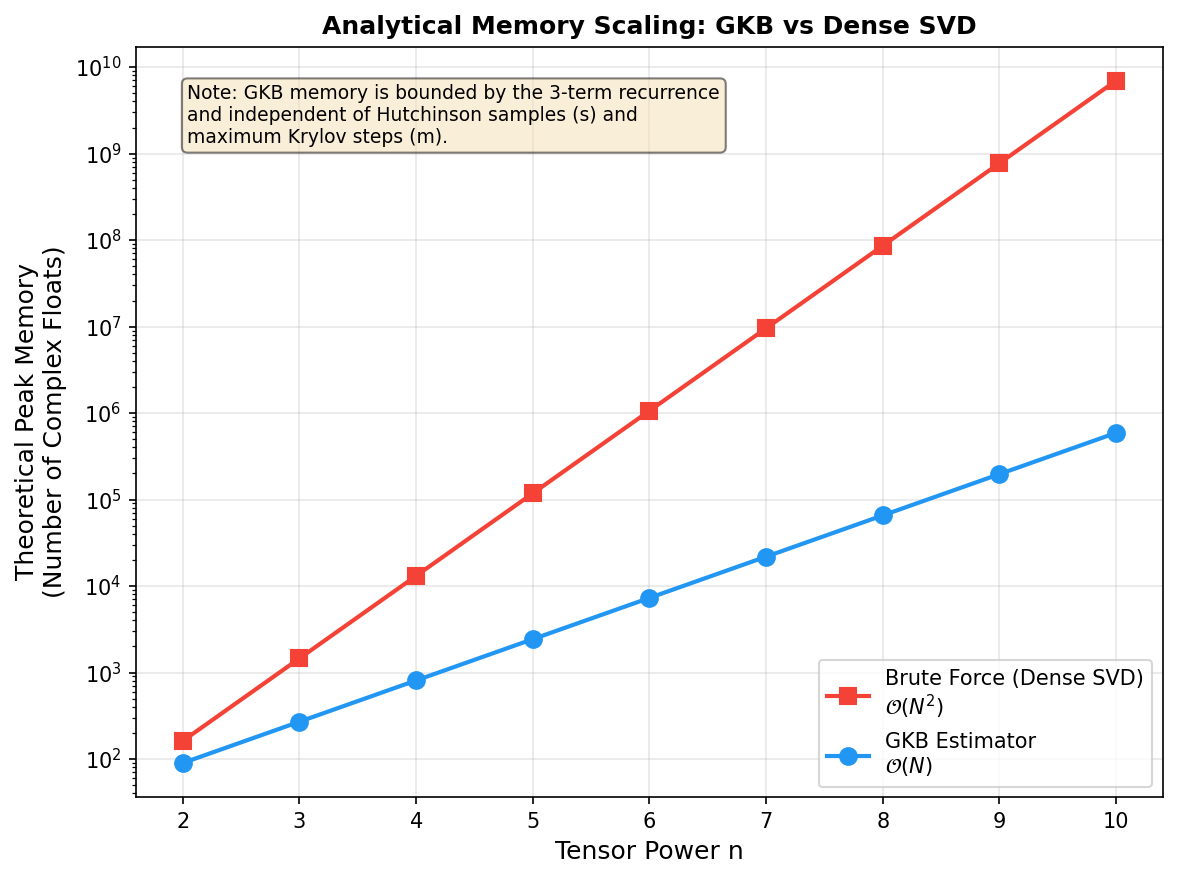
\includegraphics[height=0.65\textheight]{memory_analytical_comparison.png}
  \end{center}
\end{frame}

\begin{frame}{Possible Further Work}
  \begin{itemize}
    \item Execute exhaustive large-scale experiments.
    \item Assess robust stopping criteria for arbitrary density matrices.
  \end{itemize}
  \vspace{1.5cm}
  \begin{center}
    \Large \textbf{Thank You!}
  \end{center}
\end{frame}

\end{document}
